\section{Evaluation and Analysis}

\subsection{Dataset}
\begin{itemize}
\item Microsoft GeoLife Dataset
GeoLife Dataset published by Microsoft Research \cite{geolife1},\cite{geolife2},\cite{geolife3}. This is a GPS trajectory dataset with GPS traces of 182 users over a period of three years (from April 2007 to August 2012). 
\item Microsoft T Drive Taxicab Dataset
This is a trajectory dataset that contains one-week trajectories of 10,357 taxis published by Microsoft Research. \cite{tdrive1} ,\cite{tdrive2}
\end{itemize}
\subsection{Clustering Effectiveness}
We have shown various comparisons and result, but the main measure of clustering effectiveness that we use is the Silhouette Coefficient(SC). SC is a standard metric that shows the effectiveness of clustering. SC is based on the cohesion and the separation of clusters formed. The cohesion ( \textit{a(x)})  is defined as the average distance of x to all other vectors in the same cluster. 
The separation (\textit{b(x)}) is defined as the minimum of the average distances of x to the vectors in other clusters.
Further, the silhouette coefficient of a data point is defined as 
\begin{equation}
s(x)=\frac{b(x)-a(x)}{max(a(x),b(x))}
\end{equation}
The total silhouette coefficient of the dataset is the average over all the points given by
\begin{equation}
SC=\frac{1}{N}\sum_{i=1}^{N}s(x)
\end{equation}
\noindent Ideally, SC is between [-1,1], where values closer to 1 representing better formed clusters. 

\subsection{Individual Movement Summary}

In this section, we talk about the experiments made on the Microsoft GeoLife Dataset. These are GPS traces of around 182 users collected over a period of three years. From this data, we aim at finding the movement summary of the person which will give us insights into how that person moves and which patters appear repeatedly. In the first section we show the working of our proposed method with supporting visuals at every step explaining the rationale behind it. Further, we implemented and modified some other works from the literature to suit the problem and have discussed the results. A brief description of the methods we have compared with are given below.

\paragraph{Dynamic Time Warping}
This is a comparison made in the choice of the similarity metric that we use. We show the effects of using DTW in place of our similarity measure, keeping everything else in the algorithm exactly as it is.The DTW similarity between A and B is defined below 
\begin{equation}
D_{dtw}(A,B) =
\left\{
	\begin{array}{ll}
		0  & \mbox{if } \text{both A and B are empty} \\
		\infty & \mbox{if } \text{one of A or B is empty}\\
                \phi _d (head(A),head(B))+
                   \\min 
\left\{
	\begin{array}{ll}
		D_{dtw}(A,rest(B)), \leftarrow \text{\emph{Stretch A}}\\

		D_{dtw}(rest(A),B),\leftarrow \text{\emph{Stretch B}}\\
                D_{dtw}(rest(A),rest(B)) 
	\end{array}
\right.          \\otherwise
	\end{array}
\right.
\end{equation}

where $\phi_d(p1,p2)=L_2-dist(p1,p2)$ 
\paragraph{SWARM}
SWARM is a moving objects clustering algorithm proposed by Li \emph{et al.}\cite{Li2010}  In this algorithm they consider trajectories to be of the same cluster if they are together in similar clusters for a specific number of (not necessarily consecutive) timestamps. 
\paragraph{TRACLUS}
 TRACLUS is an algorithm proposed by Lee \emph{et al.} in \cite{Lee2007}. This algorithm partitions the trajectories, clusters the partitions and then comes up with a final representative cluster. 


\subsubsection{Proposed Method-OD}
In this section we show each stage of the proposed method and the corresponding visualizations at that stage for a test user. 
Fig. \ref{fig:alltrajs} shows all the trajectories of the user. We compute the similarity matrix using the similarity defined earlier  and run hierarchical clustering on it. 

\begin{figure}
\centering     
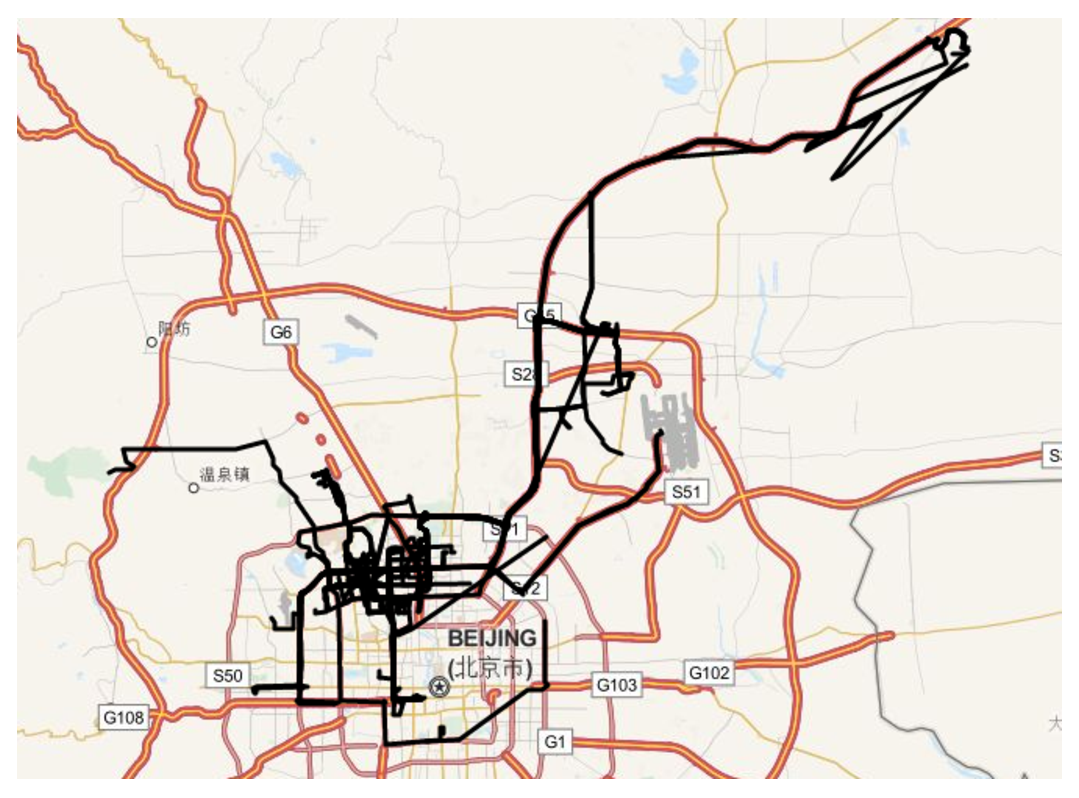
\includegraphics[scale=0.4]{figs/new/allTrajs.eps}
\caption{A snapshot of all the trajectories of the test user (363 trajectories in total)}
\label{fig:alltrajs}  
\end{figure}


The dendrogram is a pictoral representation of how similar the trajectories are among each other. The ones more similar to each other are paired closer to the bottom as compared to the ones higher in the tree. Fig \ref{fig:dendrogram} shows the dendrogram of the trajectories of the test user. The user had 363 trajectories in total, so the dendrogram has 363 leaves. 
\begin{figure}[t]
\centering     
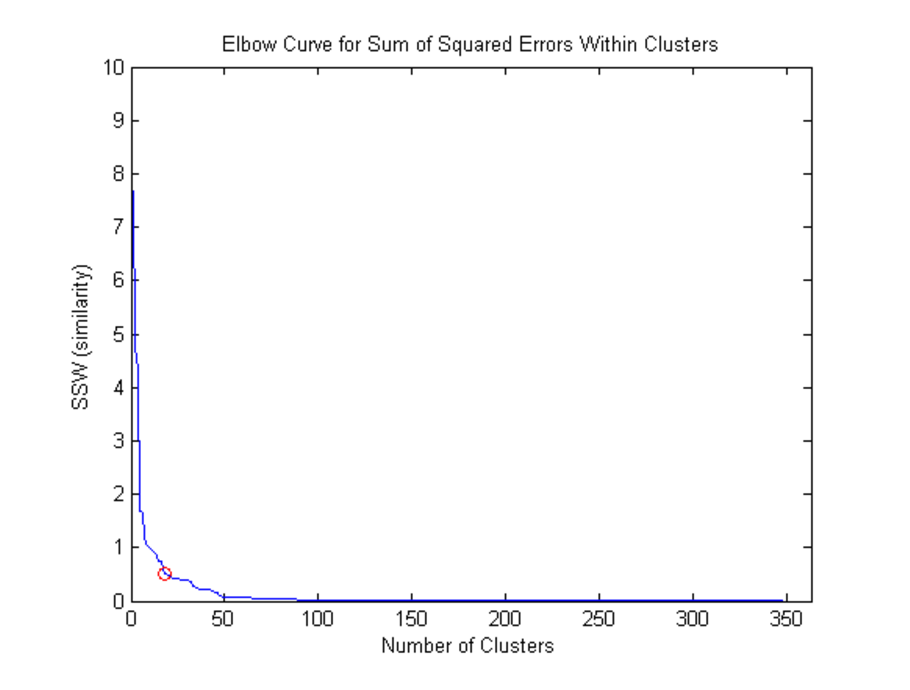
\includegraphics[scale=0.5]{figs/new/elbow.eps}
\caption{Elbow curve - Plot of the SSW vs number of Clusters; Elbow point ~ 18 clusters}
\label{fig:elbow}  
\end{figure}
\begin{figure*}
\centering     
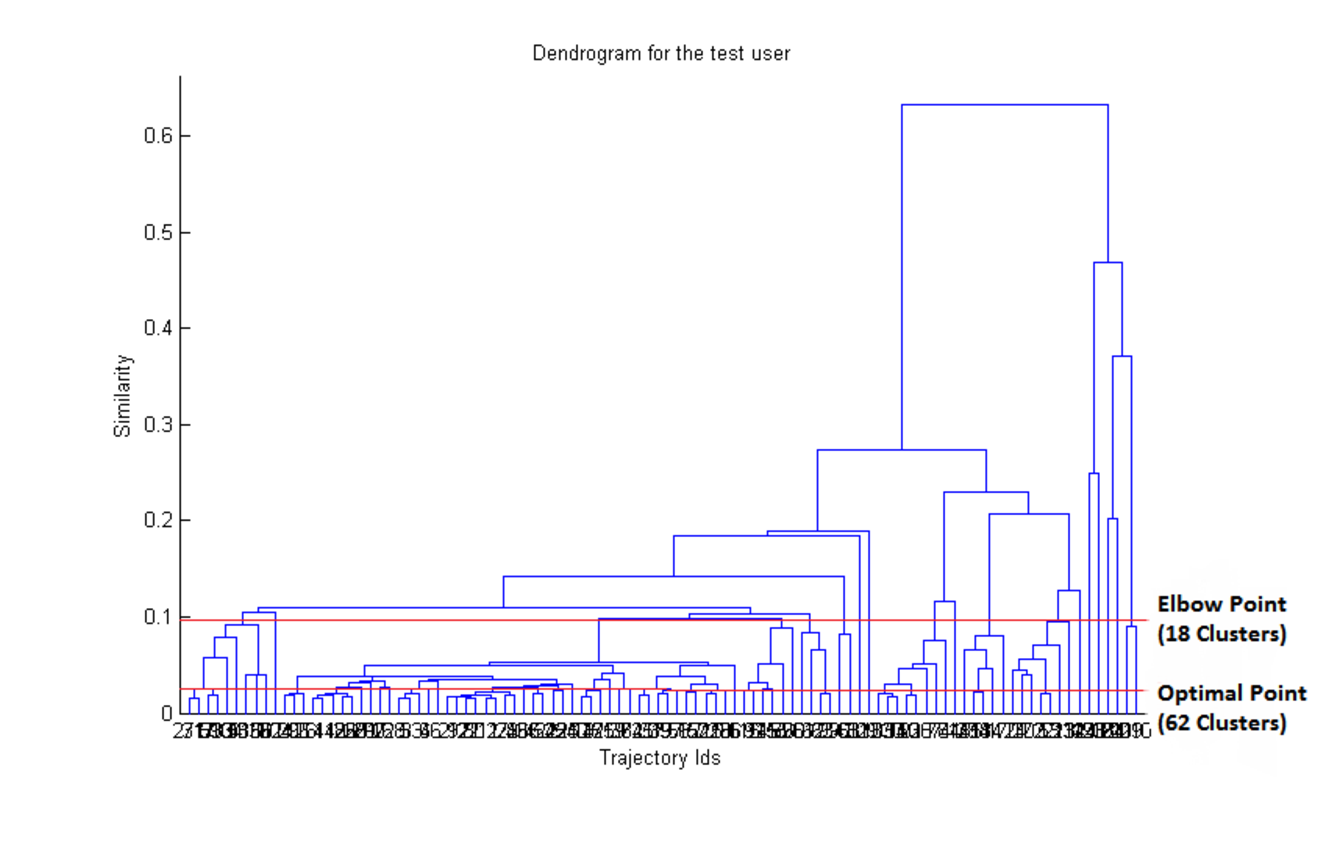
\includegraphics[scale=0.5]{figs/new/dendrogram.eps}
\caption{Dendrogram of the all the trajectories (Shows the hierarchy of similarity) The elbow point is at 18 clusters, whereas the optimal number of clusters is 62 }
\label{fig:dendrogram}  
\end{figure*}
To obtain a certain cluster of the trajectories, we have to cut the dendrogram at a certain level. The height at which we cut the dendrogram decides the number of clusters we will get. Finding the right height at which we should cut the dendrogram is one of the biggest challenges in coming up with an accurate summary for a user. One method which is widely used in literature is to plot the cumulative Sum of Squared Errors within Cluster as the cluster number varies from 1 to N. This is called the elbow curve or the scree plot and the elbow point in this curve should give us the right number of clusters. The rationale behind this is that we want to find the saturation point beyond which even on increasing the number of clusters, the error within the clusters doesnt decrease significantly. But, in our case, we found that the elbow point doesn't get us anywhere close to the actual optimal point of clustering. The validation of the clusters formed at each value of number of clusters was done by visualizing the results and looking at the general tightness of the clusters. Fig \ref{fig:elbow} shows the elbow curve with two lines indicating the elbow point, and the optimal cluster number. We see that the actual optimal point is way beyond the elbow point, and show the visualizations of the top 4 clusters at both the elbow point, in Fig. \ref{fig:elbowVisual} and (elbow point +5) number of clusters in Fig. \ref{fig:elbow5visual}.  


\begin{figure*}
    \centering
    \begin{subfigure}[t]{.5\textwidth}
        \centering
        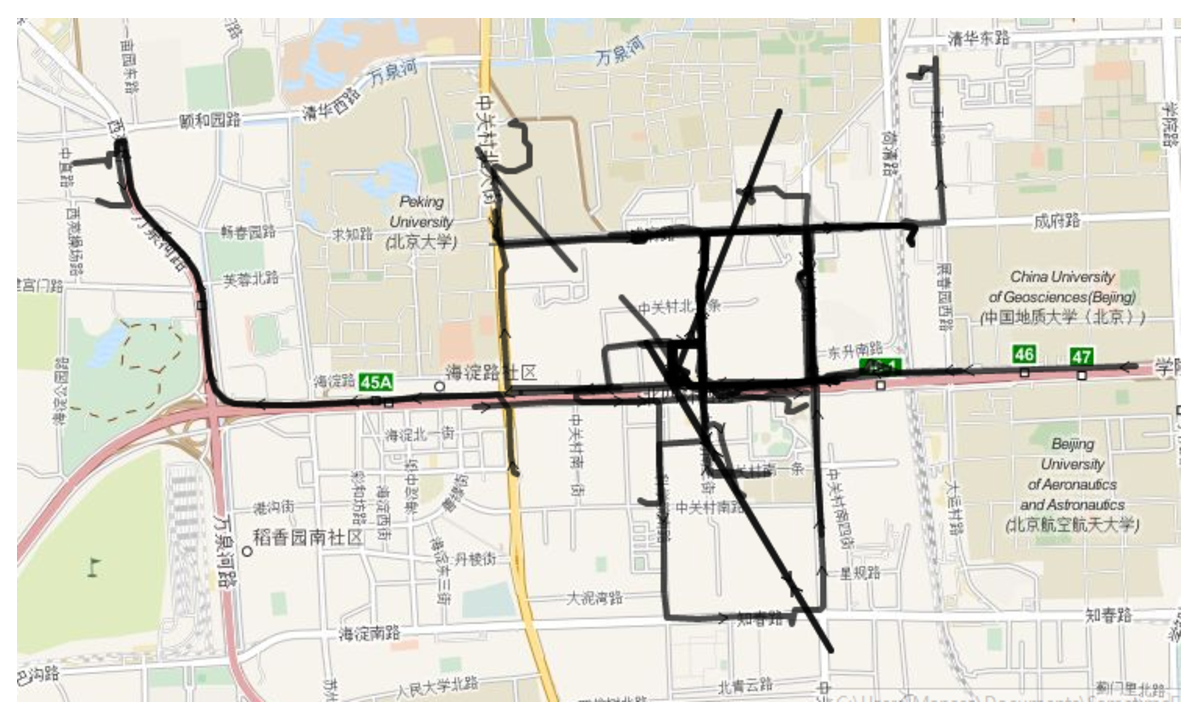
\includegraphics[width=6cm,height=4cm,keepaspectratio]{figs/new/Elbow_Cluster1.eps}
        \caption{Cluster 1 ( 32 trajectories)}
    \end{subfigure}%
    \begin{subfigure}[t]{.5\textwidth}
        \centering
        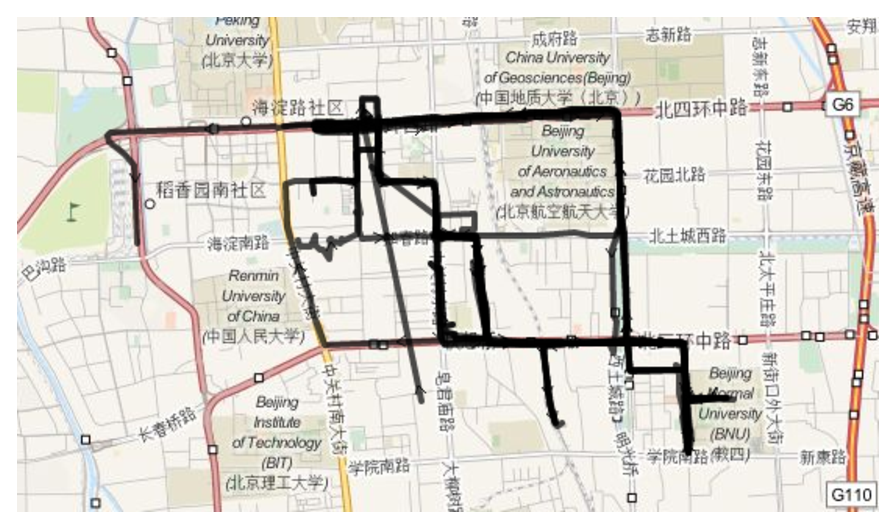
\includegraphics[width=6cm,height=4cm,keepaspectratio]{figs/new/Elbow_Cluster2.eps}
        \caption{Cluster 2(31 trajectories)}
    \end{subfigure}
        
    \begin{subfigure}[t]{.5\textwidth}
        \centering
        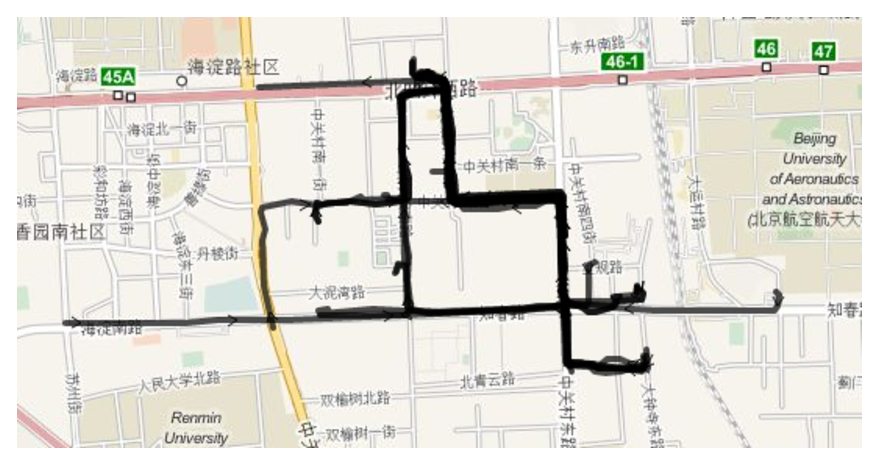
\includegraphics[width=6cm,height=4cm,keepaspectratio]{figs/new/Elbow_Cluster3.eps}
        \caption{Cluster 3(31 trajectories)}
    \end{subfigure}%
    \begin{subfigure}[t]{.5\textwidth}
        \centering
        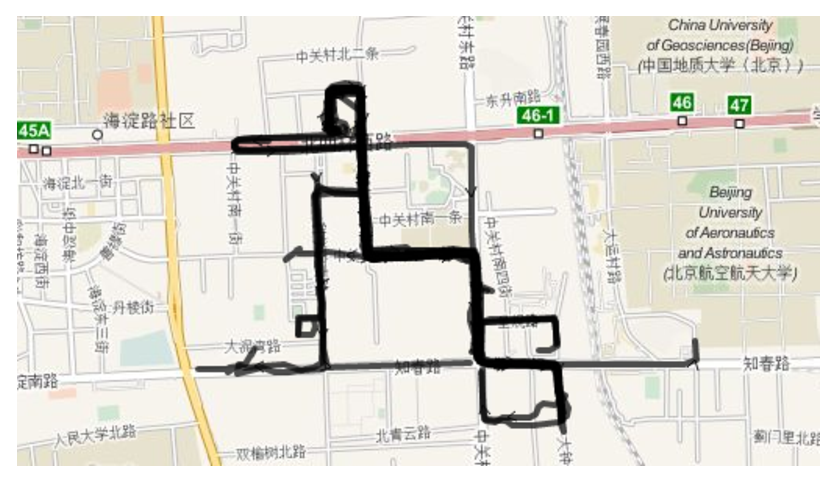
\includegraphics[width=6cm,height=4cm,keepaspectratio]{figs/new/Elbow_Cluster4.eps}
        \caption{Cluster 4(31 trajectories)}
    \end{subfigure}
    \caption{Visualizations of the top 4 clusters at Elbow Point}
    \label{fig:elbowVisual}
\end{figure*}

\begin{figure*}
    \centering
    \begin{subfigure}[t]{.5\textwidth}
        \centering
        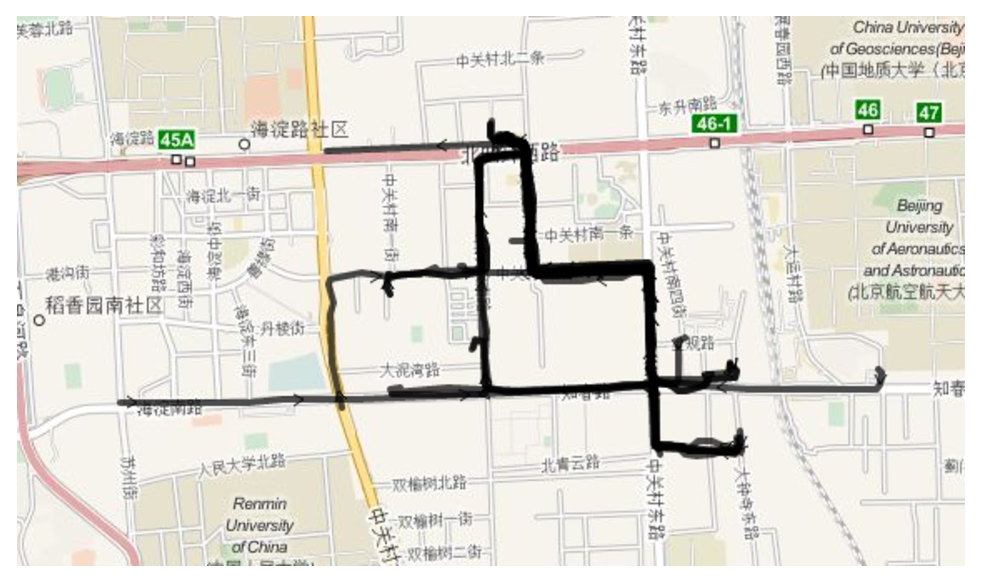
\includegraphics[width=6cm,height=4cm,keepaspectratio]{figs/new/Elbow5_Cluster1.eps}
        \caption{Cluster 1 ( 31 trajectories)}
    \end{subfigure}%
    ~ 
    \begin{subfigure}[t]{.5\textwidth}
        \centering
        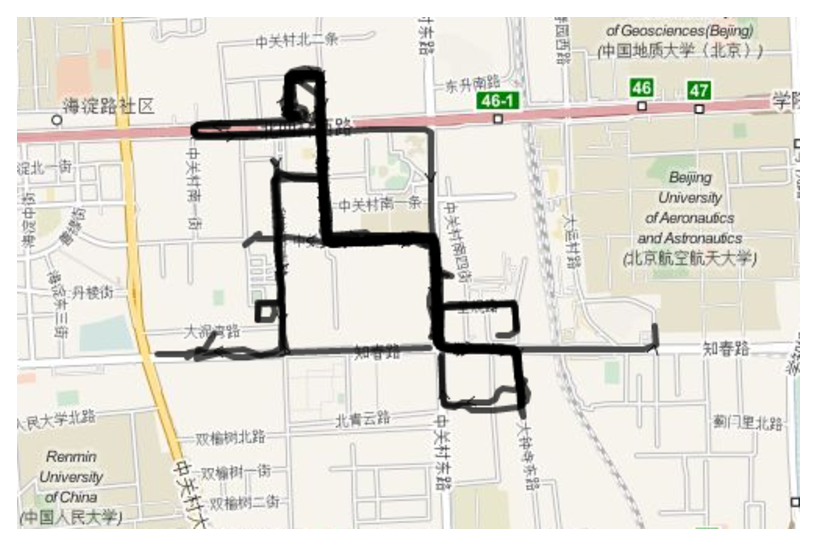
\includegraphics[width=6cm,height=4cm,keepaspectratio]{figs/new/Elbow5_Cluster2.eps}
        \caption{Cluster 2(31 trajectories)}
    \end{subfigure}
    
    \begin{subfigure}[t]{.5\textwidth}
        \centering
        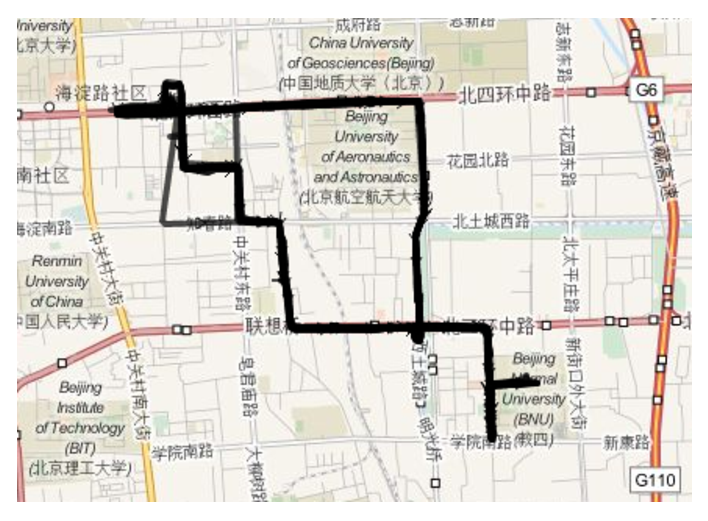
\includegraphics[width=6cm,height=4cm,keepaspectratio]{figs/new/Elbow5_Cluster3.eps}
        \caption{Cluster 3(24 trajectories)}
    \end{subfigure}%
    \begin{subfigure}[t]{.5\textwidth}
        \centering
        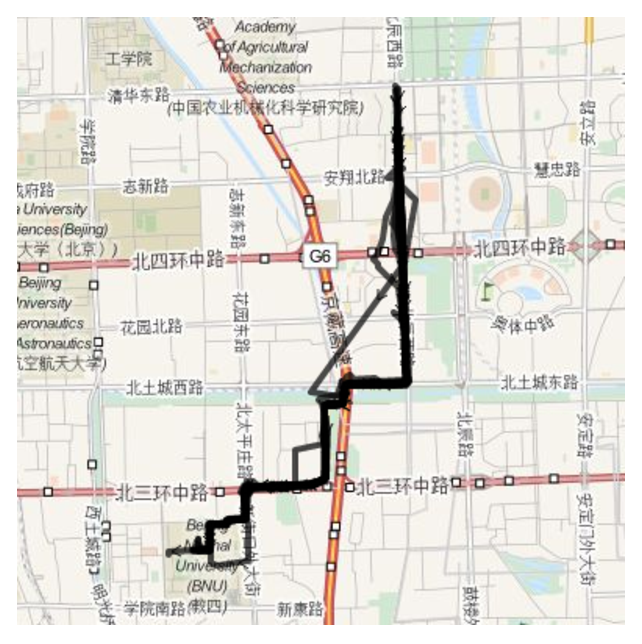
\includegraphics[width=6cm,height=4cm,keepaspectratio]{figs/new/Elbow5_Cluster4.eps}
        \caption{Cluster 4(20 trajectories)}
    \end{subfigure}
    \caption{Visualizations of the top 4 clusters at Elbow Point+5 point- Clusters not tight enough,need to go down the dendrogram further}
    \label{fig:elbow5visual}
\end{figure*}
Thus, we see that the elbow point does not get us anywhere close to the optimal number of clusters, but can help as a starting point for finding the optimal number. One insight that the elbow point gives is that the optimal point cant be before the elbow point, and hence we can prune the search space till the elbow point. 
The heuristic that we follow to obtain the optimal number of clusters is to traverse down the dendrogram , starting from the elbow point, and at any stage if we hit a cluster where the maximum pointwise distance between any pair of trajectories is less than $\delta$, we report it as a final cluster. 
\begin{figure*}
    \centering
    \begin{subfigure}[t]{.5\textwidth}
        \centering
        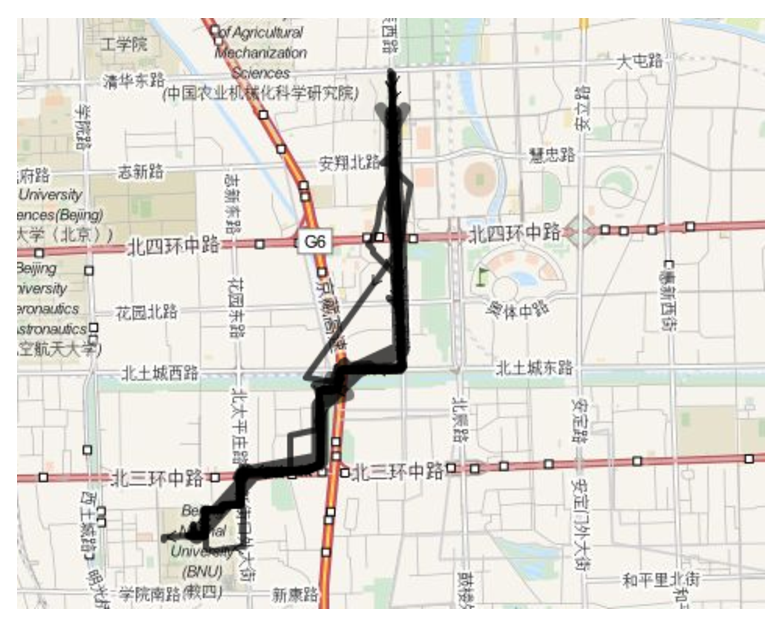
\includegraphics[width=6cm,height=4cm,keepaspectratio]{figs/new/FinalCluster1.eps}
        \caption{Cluster 1 ( 20 trajectories)}
    \end{subfigure}%
    ~ 
    \begin{subfigure}[t]{.5\textwidth}
        \centering
        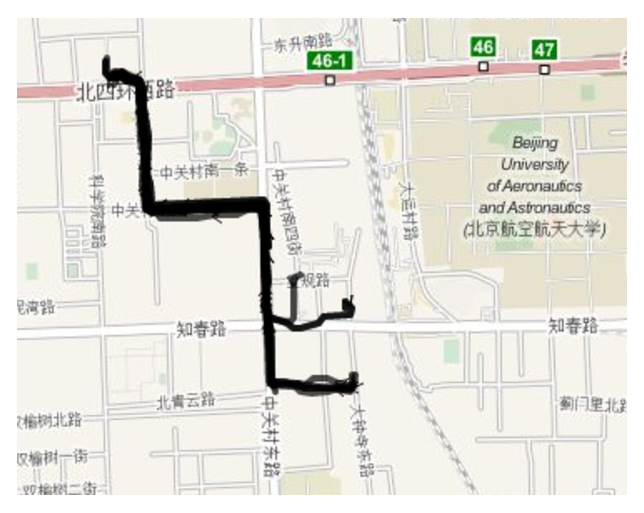
\includegraphics[width=6cm,height=4cm,keepaspectratio]{figs/new/FinalCluster2.eps}
        \caption{Cluster 2(15 trajectories)}
    \end{subfigure}
    
    \begin{subfigure}[t]{.5\textwidth}
        \centering
        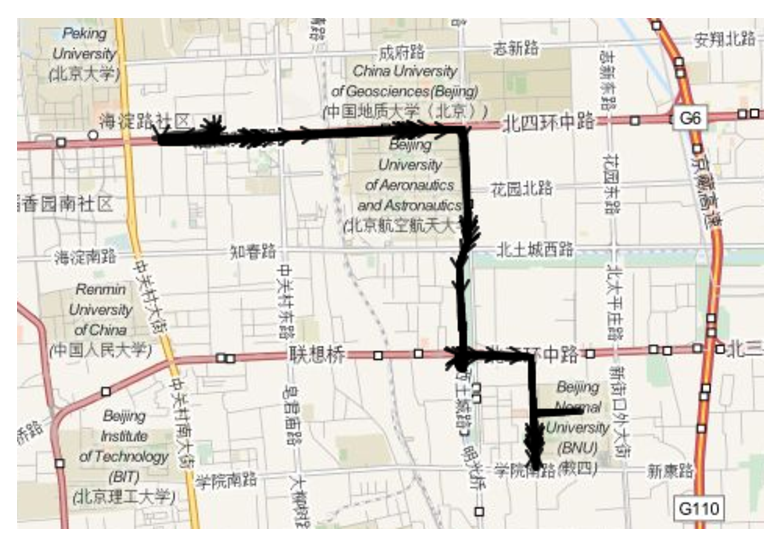
\includegraphics[width=6cm,height=4cm,keepaspectratio]{figs/new/FinalCluster3.eps}
        \caption{Cluster 3(11 trajectories)}
    \end{subfigure}%
    \begin{subfigure}[t]{.5\textwidth}
        \centering
        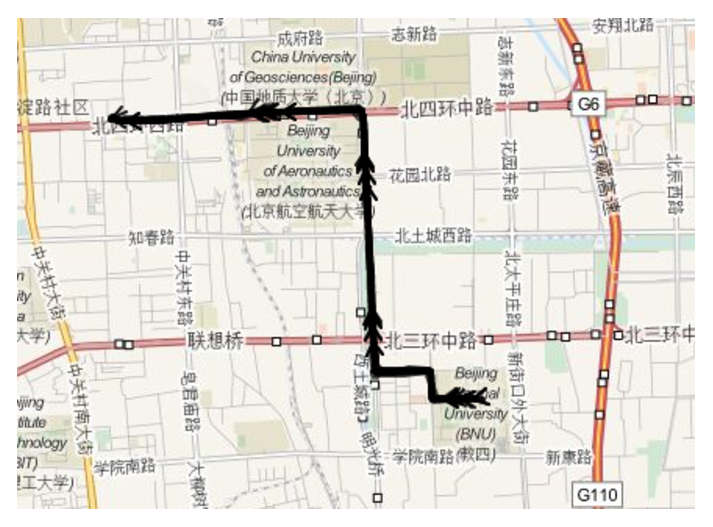
\includegraphics[width=6cm,height=4cm,keepaspectratio]{figs/new/FinalCluster4.eps}
        \caption{Cluster 4(9 trajectories)}
    \end{subfigure}
    \caption{Visualizations of the top 4 final optimal clusters}
    \label{fig:finalClusters}
\end{figure*}

Fig.\ref{fig:finalClusters} shows the visualizations of the top-4 clusters at the optimal level. 
\subsubsection{Variation with DBSCAN} 
In order to make an attempt at doing away with the heuristic, we tried another approach. In this approach we perform two stages of clustering followed by a DBSCAN based on the OD similarity measure we proposed. This method is described below : 
\begin{itemize}
\item In the first stage, we cluster the trajectories based on the Origin to origin distance. We run hierarchical clustering, and then plot the elbow curve for the SSW values and cluster it at the elbow point. 
\item In the next stage, we further cluster each cluster obtained from above based on the destination distances and performing hierarchical clustering individually on each of the clusters.
\item Once we have performed the origin and destination clusters, we now have trajectories clustered on their OD values. Now, on each of these individual clusters, we run DBSCAN based on the similarity proposed earlier. The values for minLns and epsilon are chosen using the heuristic mentioned in the paper .
\end{itemize}
By using this variant, we dont use the heuristic at any step, and are still successful in getting optimum results. The visualizations of the top 4 clusters by using this method is shown in Fig. \ref{fig:DBSCANRes}
\begin{figure*}
    \centering
    \begin{subfigure}[t]{.5\textwidth}
        \centering
        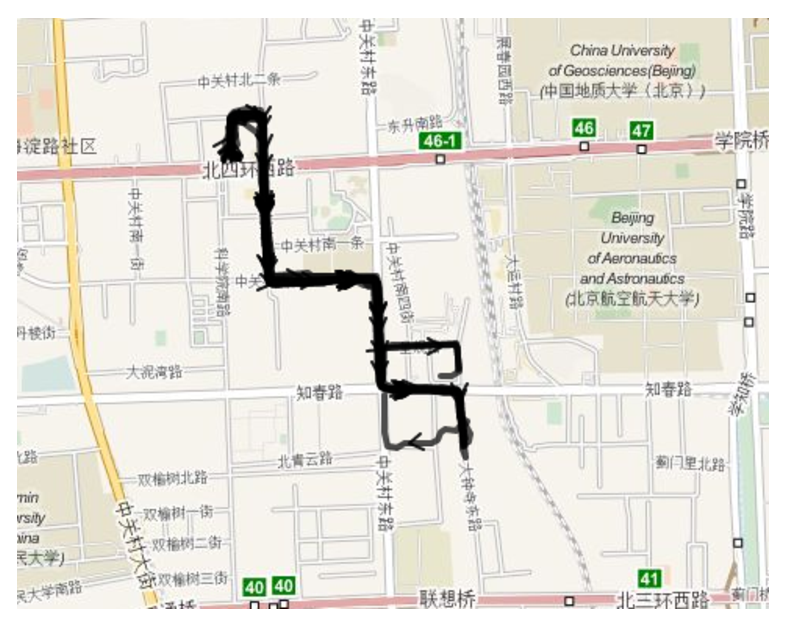
\includegraphics[width=6cm,height=4cm,keepaspectratio]{figs/new/DBSCAN1.eps}
        \caption{Cluster 1 ( 19 trajectories)}
    \end{subfigure}%
    ~ 
    \begin{subfigure}[t]{.5\textwidth}
        \centering
        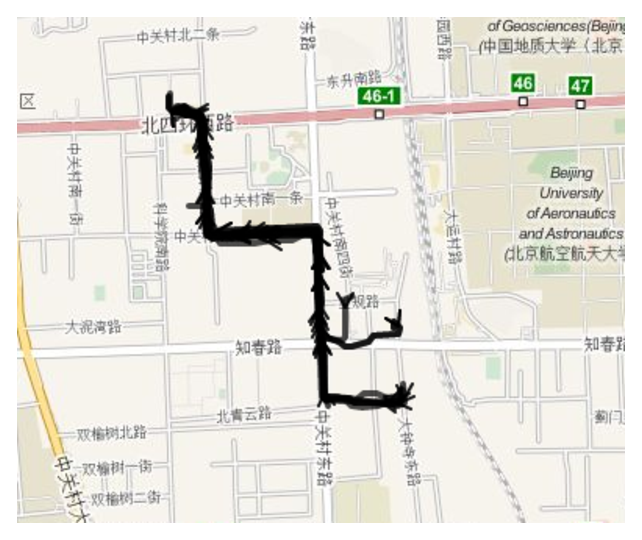
\includegraphics[width=6cm,height=4cm,keepaspectratio]{figs/new/DBSCAN2.eps}
        \caption{Cluster 2(16 trajectories)}
    \end{subfigure}
    
    \begin{subfigure}[t]{.5\textwidth}
        \centering
        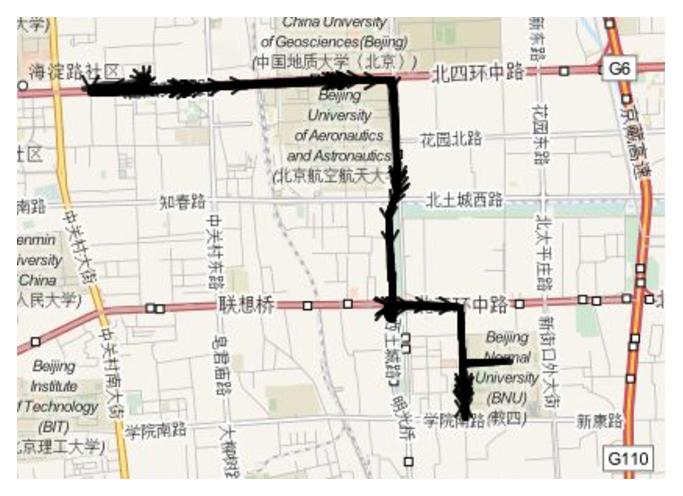
\includegraphics[width=6cm,height=4cm,keepaspectratio]{figs/new/DBSCAN3.eps}
        \caption{Cluster 3(11 trajectories)}
    \end{subfigure}%
    \begin{subfigure}[t]{.5\textwidth}
        \centering
        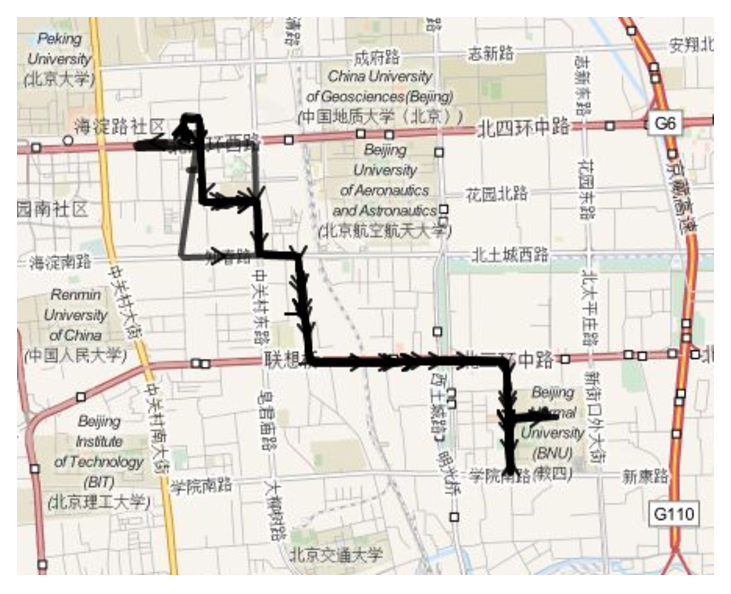
\includegraphics[width=6cm,height=4cm,keepaspectratio]{figs/new/DBSCAN4.eps}
        \caption{Cluster 4(9 trajectories)}
    \end{subfigure}
    \caption{Visualizations of the top 4 final optimal clusters using the DBSCAN variation}
    \label{fig:DBSCANRes}
\end{figure*}

\subsubsection{Comparisons with DTW}
The first comparison is made using Dynamic Time Warping as the similarity metric, and clustering based on that matrix.WE use the same framework as that proposed in our method, the only difference being that we plug in DTW similarity in place of our OD based similarity defined earlier. DTW is very close to our method considering the clustering effectiveness, but there are cases where it misses out trajectories that are a part of a meaningful trip summary. On the basis of computation time, our approach is way faster than DTW, because DTW heavily depends on the number of sample points. As the number of sample points increase, the time starts to blow up.

Problems with DTW
\begin{itemize}
\item
DTW is not a metric as it violates triangle inequality. This can lead to issues during clustering.Any distance metric d follows triangle inequality if, for any three points, x,y,and z: d(x, z) ≤ d(x, y) + d(y, z).     Figure \ref{fig:dtw_triangleineq} shows an example of the violation of triangle inequality using DTW similarity.
\begin{figure}
\centering     
\includegraphics[scale=0.5]{figs/DTW_triangle_ineq.jpg}
\caption{Example of Triangle Inequality Violation using DTW }
\label{fig:dtw_triangleineq}  
\end{figure}

\item 
The biggest concern about DTW is the computation time. When the sample points are very large, it can get to as much as 400 times slower than the proposed approach. If the points are resampled and DTW similarity is computed, it would reduce to the same as pointwise Eucledian distance, and would still be computationally more expensive. Fig \ref{fig:time_dtw_od} shows the computation time differences over all the users for clustering using  DTW and OD similarity measures over all the users

\begin{figure}
\centering     
\includegraphics[scale=0.5]{figs/dtw_od_time.eps}
\caption{Computation time comparison of DTW and OD }
\label{fig:time_dtw_od}  
\end{figure}

\item
As we decrease the number of sample points, the effectiveness of both our proposed method and DTW go down. But the goodness of the clusters returned by DTW decreases more than that of the proposed method. We reduced the number of sample points in each of the trajectories to 90\%,95\%, and 97\% and plotted the silhouette coefficient values using DTW,LP and OD. 

\begin{figure*}
    \centering
    \begin{subfigure}[t]{.5\textwidth}
        \centering
        \includegraphics[scale=0.4]{figs/noise_90_cdf.jpg}
        \caption{CDF of the silhouette coefficient for 90\% reduction of sample points }
    \end{subfigure}%
	\begin{subfigure}[t]{.5\textwidth}
        \centering
        \includegraphics[scale=0.4]{figs/noise_90_sil.jpg}
        \caption{Plot of the silhouette coefficient for 90\% reduction of sample points}
    \end{subfigure}
     \caption{90\% reduction in sample points- Comparison of silhouette graphs}
    \label{fig:noise_90}    
\end{figure*}


\begin{figure*}
    \centering
    \begin{subfigure}[t]{.5\textwidth}
        \centering
        \includegraphics[scale=0.4]{figs/noise_95_cdf.jpg}
        \caption{CDF of the silhouette coefficient for 95\% reduction of sample points }
    \end{subfigure}%
	\begin{subfigure}[t]{.5\textwidth}
        \centering
        \includegraphics[scale=0.4]{figs/noise_95_sil.jpg}
        \caption{Plot of the silhouette coefficient for 95\% reduction of sample points}
    \end{subfigure}
    \caption{95\% reduction in sample points- Comparison of silhouette graphs}
    \label{fig:noise_95}       
\end{figure*}


\begin{figure*}
    \centering
    \begin{subfigure}[t]{.5\textwidth}
        \centering
        \includegraphics[scale=0.4]{figs/noise_97_cdf.jpg}
        \caption{CDF of the silhouette coefficient for 97\% reduction of sample points }
    \end{subfigure}%
	\begin{subfigure}[t]{.5\textwidth}
        \centering
        \includegraphics[scale=0.4]{figs/noise_97_sil.jpg}
        \caption{Plot of the silhouette coefficient for 97\% reduction of sample points}
    \end{subfigure}
    \caption{97\% reduction in sample points- Comparison of silhouette graphs}
    \label{fig:noise_97}       
\end{figure*}
\end{itemize}
\subsubsection{Comparison with SWARM}
The major problems with SWARM are as follows: 
\begin{itemize}
\item Does not report all the big clusters
\item Dependent a lot on the sample points. If we resample, it would be computationally more expensive than our approach.
\end{itemize}

We show that our method performs better than SWARM over all the users using the values of the Silhouette Coefficient of the resulting clusters in Fig \ref{fig:SWARM_OD}. We also show the CDF of the SSW of the resulting clusters of SWARM vs our method in Fig \ref{fig:SSW_SWARM}.
\begin{figure*}
    \centering
    \begin{subfigure}[t]{.5\textwidth}
        \centering
        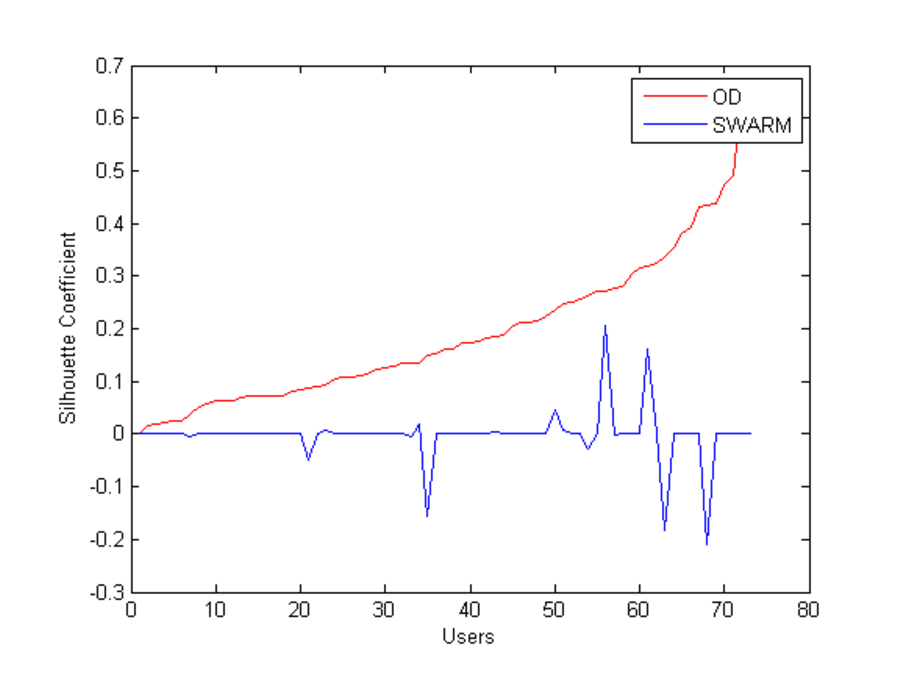
\includegraphics[scale=0.6]{figs/swarm_od_silcomparison.eps}
\caption{Silhouette Values of the resulting clusters for SWARM and OD- We perform significantly better over all users}
\label{fig:SWARM_OD}  
    \end{subfigure}%
	\begin{subfigure}[t]{.5\textwidth}
        \centering
        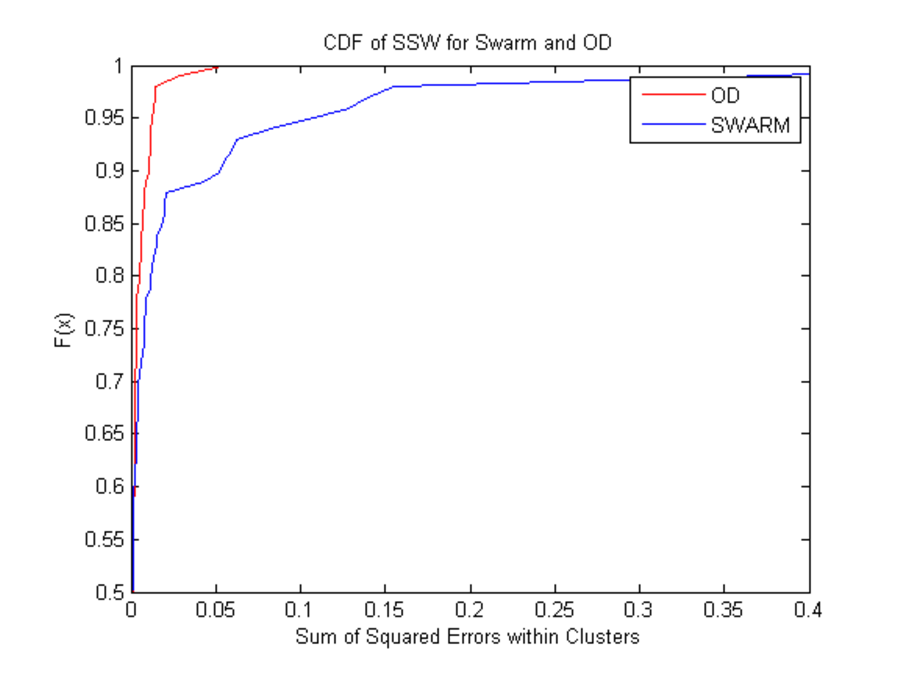
\includegraphics[scale=0.6]{figs/swarm_od_ssw.eps}
\caption{SSW Values of the resulting clusters for SWARM and OD- Our SSW error is lesser than SWARM over all users}
\label{fig:SSW_SWARM} 
    \end{subfigure}
    \caption{SWARM comparisons}
    \label{fig:swarm}       
\end{figure*}


\subsubsection{TraClus}
TraClus looks at the sub-trajectory level, and clusters trajectories on the basis of the similarities between those sub-trajectories. In the first phase, it partitions the trajectories into segments, and in the second phase, it clusters the partitions together using a DBSCAN-like technique.The problems with TrajClus are
\begin{itemize}

\item
The similarity measure between any two partitions is defined as a weighted sum of the perpendicular distance, parallel distance and the angular distance between the partitions. Here, three quantities with different units are being merged together, so when two partitions are similar, it is difficult to say which distance contributed to the similarity. Also, this creates a problem in arriving at the neighbourhood parameters. 

\item
 There are two parameters used in this algorithm, \textit{epsilon} and \textit{minLns}. \textit{epsilon} defines the neighourhood reach of each of the partition, and minLns is the minimum number of Partitions required in the neighbourhood for it to be considered as a cluster. The authors suggest a simulated annealing technique to arrive at the value of epsilon , and from that value, further calculate the value of minLns. But, because the algorithm is highly associative, nearly all the partitions end up in one cluster, thus not identifying the correct movement summaries. 
   
   
\begin{figure*}
    \centering
    \begin{subfigure}[t]{.5\textwidth}
        \centering
        \includegraphics[scale=0.4]{figs/TrajClus_full.jpg}
        \caption{All the trajectories of an example user }
\label{fig:TrajClus_full}  
    \end{subfigure}%
	\begin{subfigure}[t]{.5\textwidth}
        \centering
        \includegraphics[scale=0.4]{figs/TrajClus_cluster.jpg}
\caption{Cluster reported by TraClus}
\label{fig:TrajClus_cluster}  
    \end{subfigure}
    \caption{TraClus Final cluster reported}
    \label{fig:traclus}       
\end{figure*}


\item

TrajClus does not give enough weightage to the direction of the line segment. In cases like animal movement or hurricane movement, this makes sense, because there wont be many cases of trajectories in different directions in a flock or cluster. But when it comes to human movement pattern, directions play a very important role in determining the movement summaries of a person. TrajClus overlooks it and clusters two trajectories in different directions in the same cluster.

\begin{figure}
\centering     
\includegraphics[scale=0.3]{figs/direction.jpg}
\caption{Trajectories with different directions clustered together by TrajClus}
\label{fig:TrajClus_direction}  
\end{figure}

\end{itemize}
\subsubsection{Next Location Prediction}
Another way to test the summarization of the movement patterns is to test a query trajectory and plot its predicted next location/destination as predicted by all the methods.

The next location prediction is done by the following algorithm:
\paragraph{Explanation of the algo}
For any query trajectory, resample, and compute similarity with the median trajectories of all summary clusters. Report the one with the maximum similarity. 


Let $g(i)$ be the probability of the summary $i$. Given an input traj $t_{\operatorname{in}}$, compute the distance (in meters or so) $d(i,t_{\operatorname{in}})$ between summary $i$ and $t_{\operatorname{in}}$. Now the probability that this sub-trajectory lies within summary $i$ is given by
\begin{eqnarray}
p(i,t_{\operatorname{in}}) = \frac{1}{\sqrt{2 \pi} \sigma_{t}} \mathrm{e}^{-0.5 \left( \frac{d(i,t_{\operatorname{in}})}{\sigma_{t}} \right)}
\end{eqnarray}
Here we assume that the input trajectory is a noisy input from GPS samples. $\sigma_{t}$ is the standard deviation of the sub-trajectory distance. For now take, $\sigma_{t} = \sigma_{p}$, where $\sigma_{p}$ is the standard deviation of the GPS sampling a location (value is 15.61, which is the 95-th percentile of GPS considering 30 m error). It should ideally be standard deviation introduced when we compute distance between 100 points of a path

For each of the methods compared, we plot the CDF of the error of the predicted destination for the Top-3 Closest clusters to each of the query trajectories. Each of the graphs contain 4 plots, each one varying the number of sample points given to the query trajectory. We have plotted the errors for query trajectories with 10\%, 25 \%, 50\% and 90\% of the sample points. 

\begin{figure*}
    \centering
    \begin{subfigure}[t]{.5\textwidth}
        \centering
        \includegraphics[scale=0.4]{figs/dtw_top.jpg}
        \caption{CDF of error in predicted destination for 1st closest cluster using DTW}
    \end{subfigure}%
	\begin{subfigure}[t]{.5\textwidth}
        \centering
        \includegraphics[scale=0.4]{figs/dtw_top2.jpg}
        \caption{CDF of error in predicted destination for 2nd closest cluster using DTW}
    \end{subfigure}
    \begin{subfigure}[t]{.5\textwidth}
        \centering
        \includegraphics[scale=0.4]{figs/dtw_top3.jpg}
        \caption{CDF of error in predicted destination for 3rd closest cluster using DTW}
    \end{subfigure}
    \caption{CDF of the error in predicted destinations for the top 1,2,3 closest clusters for \emph{DTW}}
    \label{fig:nextloc_DTW}       
\end{figure*}

\begin{figure*}
    \centering
    \begin{subfigure}[t]{.5\textwidth}
        \centering
        \includegraphics[scale=0.4]{figs/od_top.jpg}
        \caption{CDF of error in predicted destination for 1st closest cluster using OD}
    \end{subfigure}%
	\begin{subfigure}[t]{.5\textwidth}
        \centering
        \includegraphics[scale=0.4]{figs/od_top2.jpg}
        \caption{CDF of error in predicted destination for 2nd closest cluster using OD}
    \end{subfigure}
    \begin{subfigure}[t]{.5\textwidth}
        \centering
        \includegraphics[scale=0.4]{figs/od_top3.jpg}
        \caption{CDF of error in predicted destination for 3rd closest cluster using OD}
    \end{subfigure}
    \caption{CDF of the error in predicted destinations for the top 1,2,3 closest clusters for \emph{OD}}
    \label{fig:nextloc_OD}       
\end{figure*}

\begin{figure*}
    \centering
    \begin{subfigure}[t]{.5\textwidth}
        \centering
        \includegraphics[scale=0.4]{figs/lp_top.jpg}
        \caption{CDF of error in predicted destination for 1st closest cluster using LP}
    \end{subfigure}%
	\begin{subfigure}[t]{.5\textwidth}
        \centering
        \includegraphics[scale=0.4]{figs/lp_top2.jpg}
        \caption{CDF of error in predicted destination for 2nd closest cluster using LP}
    \end{subfigure}
   \caption{CDF of the error in predicted destinations for the top 1,2 closest clusters for \emph{LP}}
    \label{fig:nextloc_LP}       
\end{figure*}

\begin{figure*}
    \centering
    \begin{subfigure}[t]{.5\textwidth}
        \centering
        \includegraphics[scale=0.4]{figs/swarm_top.jpg}
        \caption{CDF of error in predicted destination for 1st closest cluster using SWARM}
    \end{subfigure}%
	\begin{subfigure}[t]{.5\textwidth}
        \centering
        \includegraphics[scale=0.4]{figs/swarm_top2.jpg}
        \caption{CDF of error in predicted destination for 2nd closest cluster using SWARM}
    \end{subfigure}
   \caption{CDF of the error in predicted destinations for the top 1,2 closest clusters for \emph{SWARM}}
    \label{fig:nextloc_SWARM}       
\end{figure*}


Some of the observations from the next location prediction results are as follows:\\
Our Approach and LP predict the destination of \emph{82\%} of the trajectories with less than 10km error for closest cluster. 
DTW also is very close with prediction \emph{80\%} of the trajectories, but SWARM fares very badly with just \emph{5\%} of the trajectories' destination predicted. SWARM cannot detect the third closest cluster for any of the input trajectories. 



%Extra Graphs --->
%\begin{figure}
%\centering     
%\includegraphics[scale=0.3]{figs/testing_sil.jpg}
%\caption{Comparison of silhouette coefficients for different schemes: OD- and LP-based clustering outperform existing mechanism. }
%\label{fig:sil_cdf}  
%\end{figure}
%
%The CDF plot shows that  DTW is very similar to our approach in terms of clustering effectiveness, but SWARM does a very poor job. 
%
%\subsubsection{Average Trajectories Per Cluster}
%Number of clusters with large number of trajectories in it is better (Figure~\ref{fig:avg_cdf} and ~\ref{fig:avgtop_cdf}). 
%
%\begin{figure}[H]
%\centering     
%\includegraphics[scale=0.3]{figs/avg.jpg}
%\caption{CDF of Average trajectories per cluster for LP-DTW-OD}
%\label{fig:avg_cdf}  
%\end{figure} 
%
%\begin{figure}[H]
%\centering     
%\includegraphics[scale=0.3]{figs/avgtop.jpg}
%\caption{CDF of Average trajectories per top-k clusters for LP-DTW-OD}
%\label{fig:avgtop_cdf}  
%\end{figure} 
%
%\subsection{Computation Time}
%
%\begin{figure}[H]
%\centering     
%\includegraphics[scale=0.3]{figs/time_log.jpg}
%\caption{Computation time  for LP-DTW-OD}
%\label{fig:time_cdf}  
%\end{figure} 
%
%
%



%\subsubsection{Visualization at various granularity }
%%\rednote {Remove later if needed}
%
%\begin{figure*}
%\centering   
%\includegraphics[scale=0.6]{figs/demo.jpg}
%\caption{Visualization at various zoom levels}
%\label{fig:demo}  
%\end{figure*}
%
%\subsubsection{Case Study: Reported Final Clusters from each method}
%
%We take up a sample case, and show the snapshots of the final clusters as reported by all the different methods. DTW and OD have similar final clusters whereas SWARM reports only final clusters. 
%
%
%\begin{figure}
%\centering     
%\includegraphics[scale=0.4]{figs/snapshot_swarm.jpg}
%\caption{Snapshot of clusters reported by SWARM }
%\label{fig:casestudy_swarm}  
%\end{figure} 
%
% 
%\begin{figure}
%\centering     
%\includegraphics[scale=0.4]{figs/snapshot_od.jpg}
%\caption{Snapshot of clusters reported by OD}
%\label{fig:casestudy_od}  
%\end{figure} 
%
%\begin{figure}
%\centering     
%\includegraphics[scale=0.4]{figs/snapshot_dtw.jpg}
%\caption{Snapshot of clusters reported by DTW}
%\label{fig:casestudy_dtw}  
%\end{figure} 
%
%\iffalse
%The table below shows the statistics of the top k clusters and the number of trajectories 
%
%\begin{table*}
%	\centering
%		\begin{tabular}{|c|c|c|c|c|} 
%			\hline
%			Method&DTW&SWARM&TrajClus&OD\\
%			\hline
%			Number of Clusters Reported&1&4&0&18\\
%			Number of trajectories in top 3 Clusters & 5&36,15,13&0&38,37,29\\
%			\hline
%		\end{tabular}
%	\caption{Comparison for case study}
%	\label{tab:case_study}
%\end{table*}
%\fi

